\chapter{Misure di Potenza}
La potenza istantanea è descritta come:
\begin{equation*}
    P = V \cdot I
\end{equation*}
Mentre il tipo di potenza che è di nostro interesse è la potenza media, definita come:
\begin{equation*}
    \frac{1}{T} \int_0^T P(t) dt
\end{equation*}
In continua, potenza media e potenza istantanea coincidono e questa condizione ci è utile quando saliamo in frequenza dato che tendenzialmente misureremo potenza nel regime sinusoidale, in cui la potenza attiva diventa:
\begin{equation*}
    P = V \cdot I cos(\varphi)
\end{equation*}
In questo tipo di regime vi è anche una parte reattiva:
\begin{equation*}
    Q = V \cdot I sin(\varphi)
\end{equation*}
Ed è legata alla potenza attiva tramite la potenza apparente:
\begin{equation*}
    P_A = \sqrt{P^2 + Q^2}
\end{equation*}

\section{Wattmetri ad Effetto Hall}
\begin{center}
    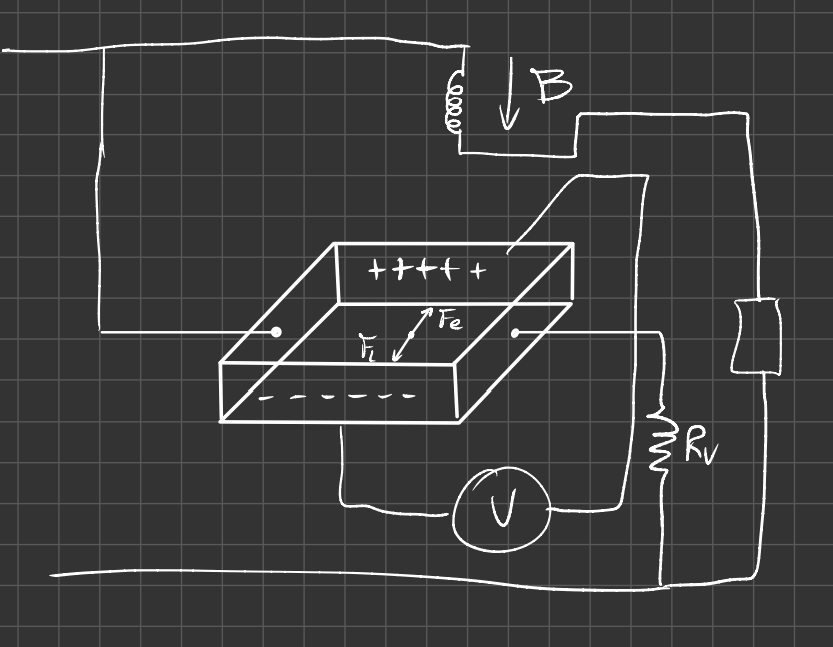
\includegraphics[width=.7\textwidth]{Images/figure48.png}
\end{center}
Come noto, in un \textbf{trasduttore} ad effetto \textbf{hall}, la tensione $V_H$ (t) è proporzionale al prodotto di due grandezze variabili:
\begin{equation*}
    V_H (t) = R_H \cdot i(t) \cdot B(t)
\end{equation*}
Dove:
\begin{itemize}
    \item $R_H$ = \textbf{costante di Hall};
    \item $i(t)$ = corrente che passa attraverso il \textbf{trasduttore};
    \item $B(t)$ = \textbf{induzione magnetica}
\end{itemize}
La \textbf{potenza} P è determinata misurando $V_H (t)$ attraverso un \textbf{voltmetro} a valor medio con alte impedenze di ingresso e considerando che $V_x (t) = a \cdot i(t)$ e $i_x (t) = b \cdot B(t)$, dove \textbf{a} e \textbf{b} sono costanti di proporzionalità:
\begin{equation*}
    P = \frac{1}{T} \int_0^T V_x (t) \cdot i_x (t) dt =  \frac{ab}{T} \int_0^T i(t) B(t) dt = R_H \cdot V_H
\end{equation*}
Dove T è il periodo del misurando.\\ \\
Nella configurazione abituale del \textbf{moltiplicatore} \textbf{di} \textbf{Hall}, l'\textbf{induzione} \textbf{Magnetica} è proporzionale alla \textbf{corrente} sul \textbf{carico} e la \textbf{corrente} di \textbf{polarizzazione} ottimale $i_v$ è fissata da un \textbf{resistore} $R_v$.
\section{Wattmetri Termici}
\begin{center}
    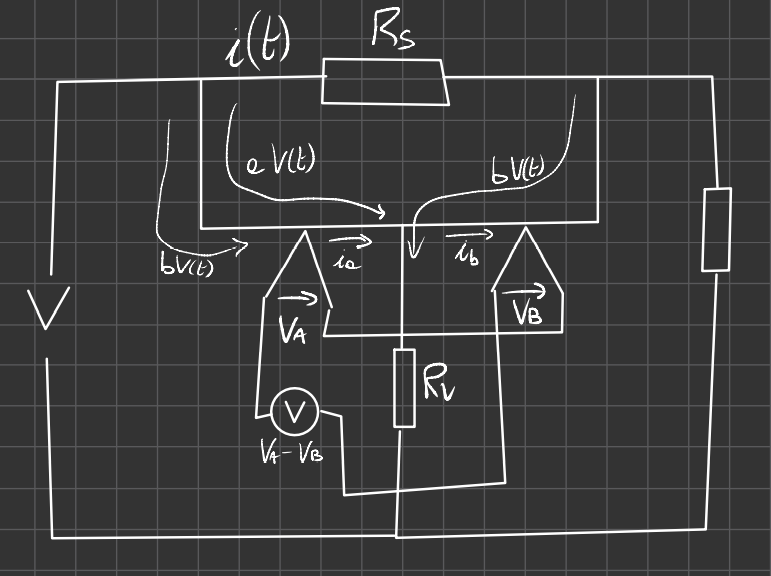
\includegraphics[width=.7\textwidth]{Images/figure49.png}
\end{center}
Il \textbf{Principio} del \textbf{Wattmetro} \textbf{Termico} è nell'uso di due \textbf{termocoppie}, la \textbf{potenza} \textbf{attiva} \textbf{P} è ottenuta tramite una misura della \textbf{tensione} \textbf{continua}  tra le due \textbf{termocoppie}.\\ \\
Adattando soluzioni basate su tecniche di \textbf{retroazione}, non sono necessarie correzioni per compensare la \textbf{non} \textbf{linearità} delle \textbf{termocoppie} e, utilizzando due \textbf{termocoppie} \textbf{gemelle} si ottiene un notevole \textbf{miglioramento} delle prestazioni.\\ 
